\section{Data Understanding}\label{sec:data_understanding}

\subsection{Question 1 – Profile of repeating students in PISA. Which variables contribute to explaining their performance in mathematics? How has it evolved over the different assessment cycles?}

For this question, we used the Student Questionnaire data from 2022. (*citar fonte*).

This dataset contains information about the students' backgrounds, their attitudes towards mathematics, and their performance in the PISA assessment. It has 1278 columns, from which 1260 are numerical and 18 are categorical.
It has 613744 rows, where each row corresponds to a student. Around 10\% of this students are repeating students, which means they have been retained in the same grade for at least one year.
In Figure \ref{fig:grade_distribution} we can see the distribution of students by grade repetition status.

\begin{figure}
    \centering
    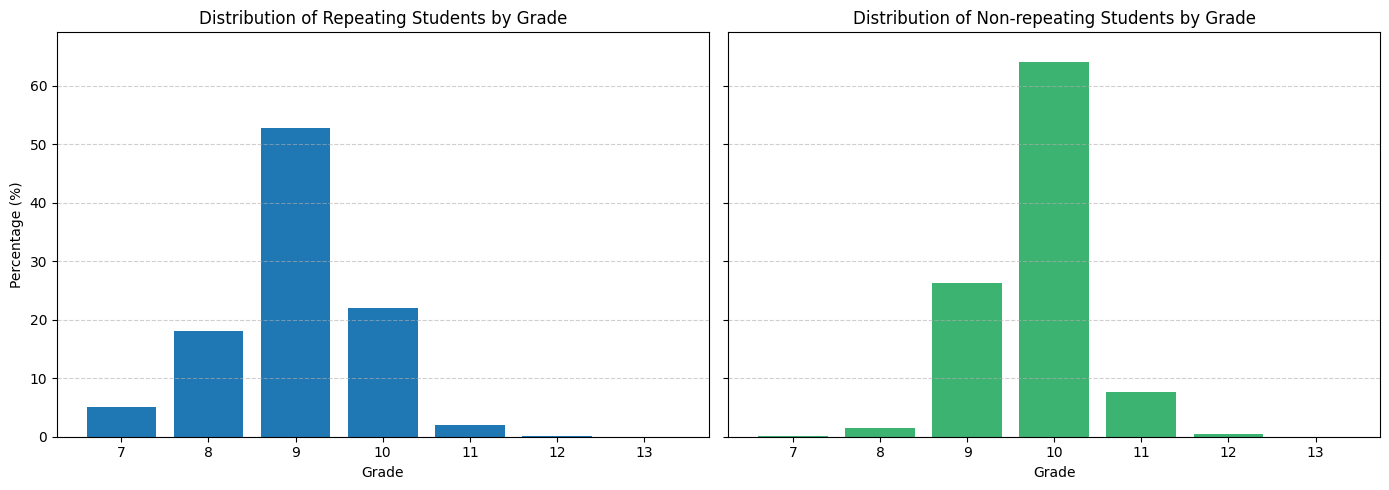
\includegraphics[width=0.48\textwidth]{figures/Q1_GradeDistribution.png}
    \caption{Distribution of students by grade repetition status.}
    \label{fig:grade_distribution}
\end{figure}

The target variable for this analysis is the student's performance in mathematics. Their score can be calculated as the average of the values across all "Possible Math Value" columns, which are represented in the dataset from \texttt{PV1MATH} to \texttt{PV10MATH}. These features are plausible values, each representing multiple estimates of the student's performance. Averaging them provides a more reliable and comprehensive measure of the student's grade.
This score is a continuous variable, and can vary from a minimun of 0 and a maximum of 1000.

We then conducted an exploratory analysis of the dataset to identify relevant patterns and potential outliers. This helped us uncover special cases that may influence student performance, such as differences in educational systems across countries.
For instance, the English school system has a different structure compared to the rest of the world (*citar fonte*), which may affect the results.
In Figure \ref{fig:country_distribution}, we can see that most of the students in 11th, 12th and 13th grades are from the UK. This difference may lead to a disproportionate representation of students and we should consider them as an exception in the next phases.

\begin{figure}
    \centering
    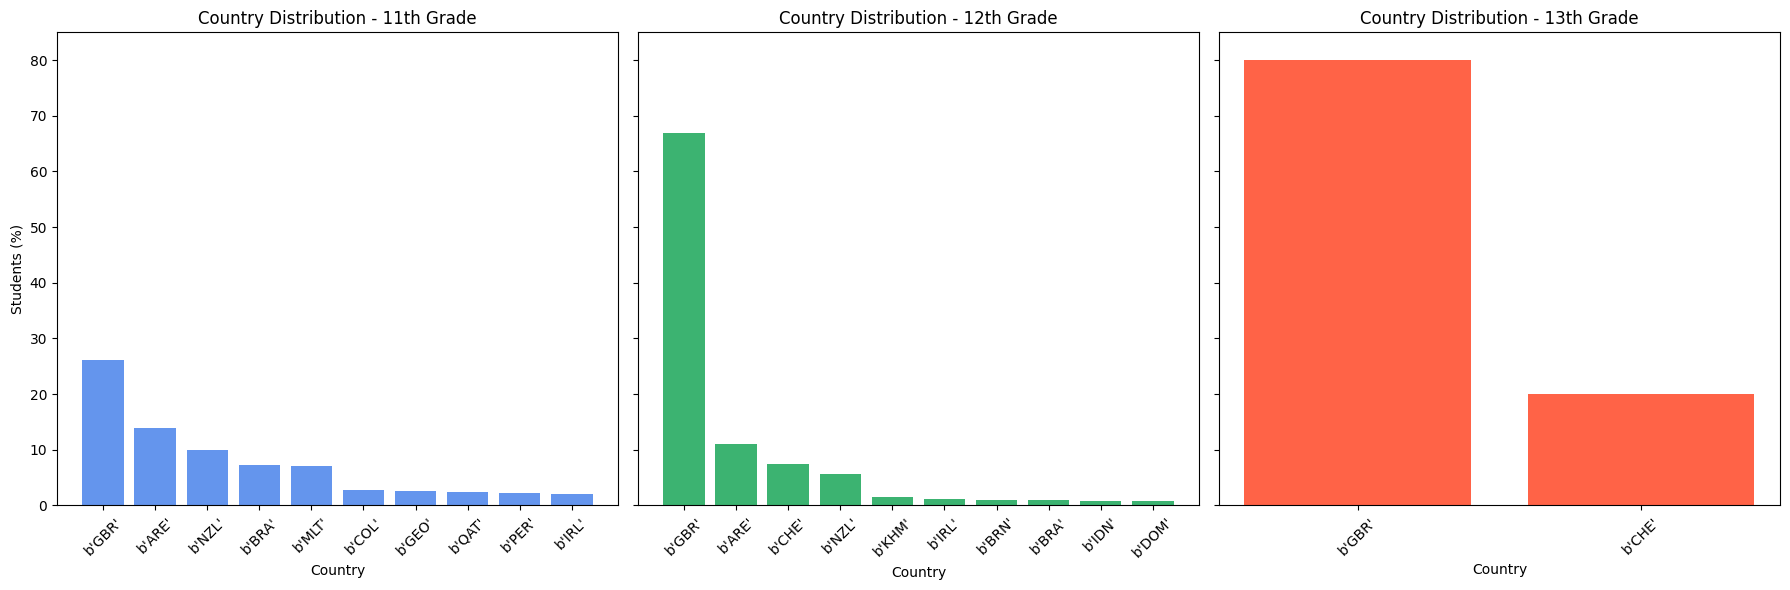
\includegraphics[width=0.48\textwidth]{figures/Q1_CountryDistri.png}
    \caption{Distribution of students by country (\%).}
    \label{fig:country_distribution}
\end{figure}

For the categorical values, we excluded country-specific and redundant variables to reduce dimensionality and focus on global trends, retaining only "CNT" (Country), which will be grouped into broader regions for future analysis.

Finally, in the last step, we verified the quality of the data. We found that some columns had a high percentage of missing values, which could affect the analysis. There were a total of 369 columns that had more than 70\% of missing values.
We also checked for duplicate rows and columns in the data, but luckily we didn't find any.

\subsection{Question 2}

\subsection{Question 3}